The proposal consist on a possibilistic valid-time model. The representation and the querying are explained in the following subsections.

\subsection{Representation of ill-known valid-time intervals}
Valid time is usually represented as an interval. The interval has a starting and an ending points. An ill-known valid-time interval is an interval in witch one or both points are ill-known. 

\begin{definition}
A Possibilistic Valid-Time Period \textbf{PVP} is a possibilistic interval defined by means of two ill-known points, namely $\left[ X,\ Y \right]$
\begin{equation}
PVP = \left[X,\ Y \right] 
\end{equation}
$X$ and $Y$ are ill-known values in the set of the real numbers $\mathbb{R}$. The uncertainty about the values taken by $X$ and $Y$ are given by the possibility distributions $\pi_X$ and $\pi_Y$.
\end{definition}

The possibility distributions $\pi_X$ and $\pi_Y$ are given in the way of a triangular distribution, as explained in subsection \ref{subsec:fuzzy-numbers}. This representation allows overlapping (Fig. \ref{fig:pvp}).


\begin{figure}[h!]
  \centering
%  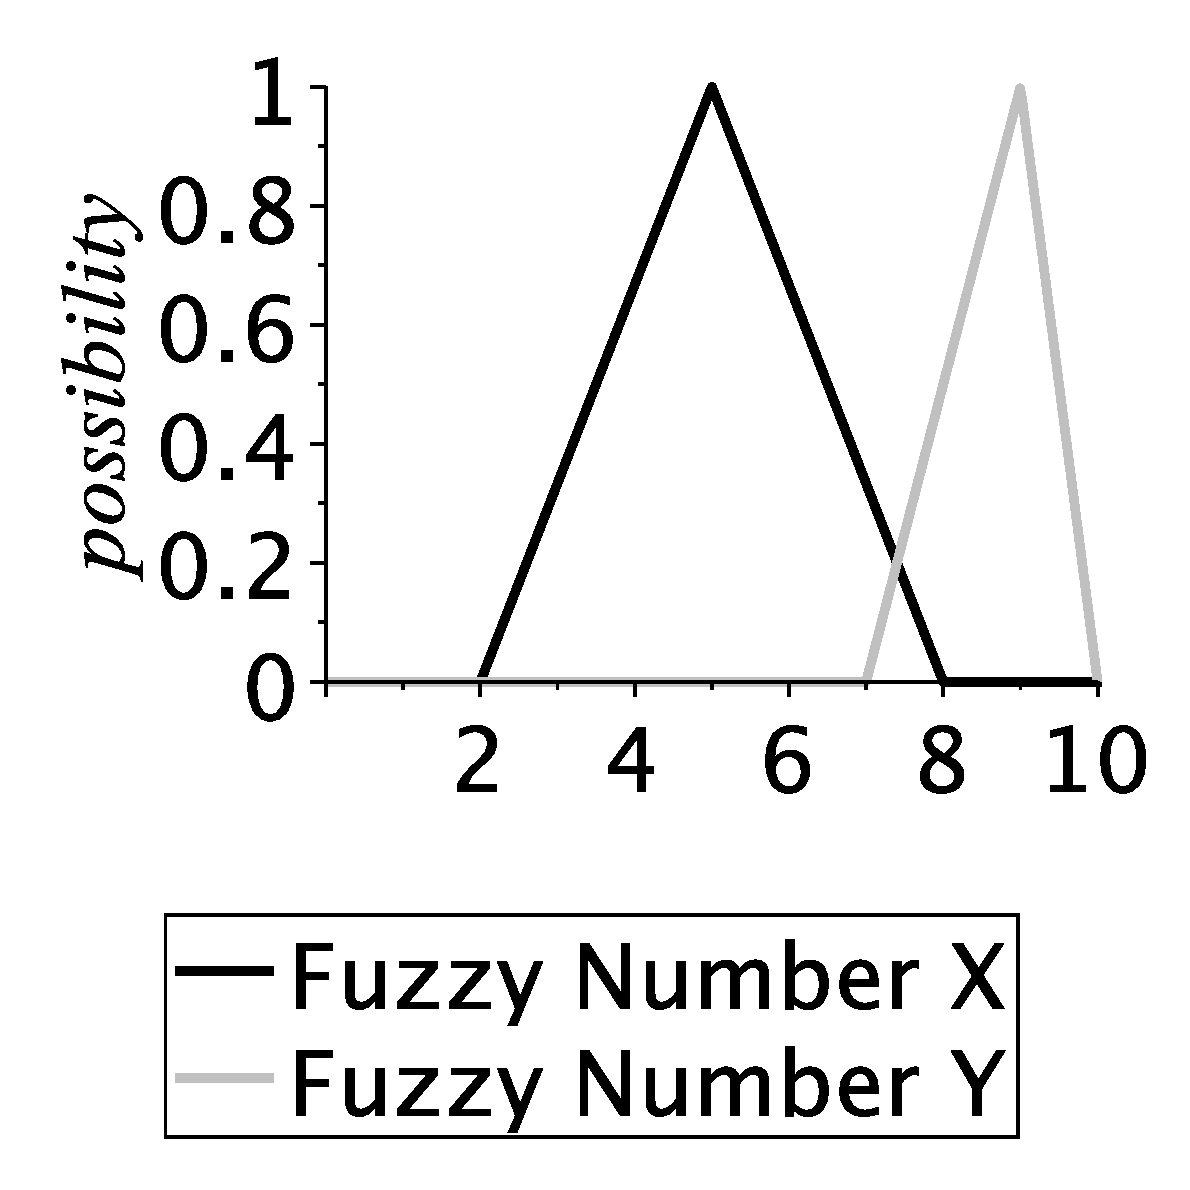
\includegraphics[scale=0.2]{graphs/2_triangular.eps}
  \caption{Two fuzzy numbers $X$ and $Y$ denoting a Possibilistic Valid-Time Period \emph{PVT}.}
  \label{fig:pvp}
\end{figure}

\subsection{Storage of valid-time intervals}
Each database row containing a \emph{PVP} stores it as two triangular possibility distributions. In our approach we propose the representation of that as proposed in the  fuzzy interface for relational databases \emph{FIRST}~\cite{Medina94gefred.a,Gal98}. In this representation it is also possible to represent not only fuzzy numbers but fuzzy constants (see table \ref{table:relational-representation-pvp}):

\begin{itemize}
\item
\emph{NULL}: This constant refers to a completely ignorance about the value. The possibility distribution for a given fuzzy number $X$ is not defined, therefore, any comparison between a fuzzy number and the \emph{NULL} constant always returns $0$.
\item
\emph{UNKNOWN}: The point has a value but it is unknown. The possibility distribution for a given fuzzy number $X$ is $\pi_X=1$
\item
\emph{UNDEFINED}: The point does not have a value. The possibility distribution for a given fuzzy number $X$ is $\pi_X=0$
\end{itemize}


\begin{table}
\caption{Relational representation for a Possibilistic Valid-Time Period.}
\centering
\begin{tabular}{c c c c c c}
\hline
Value & FT & F1 & F2 & F3  \\ \hline
UNKNOWN & 0 & NULL & NULL & NULL  \\ 
UNDEFINED & 1 & NULL & NULL & NULL  \\ 
NULL & 2 & NULL & NULL & NULL  \\ 
$\left[D,\ a,\ b \right]$ & 3 & $D$ & $D-a$ & $D+b$ \\ 
\hline
\end{tabular}
\label{table:relational-representation-pvp}
\end{table}

\subsection{Querying ill-known valid-time intervals}
In order to provide a complete model, we will provide the tools for querying. This allows the user to specify both the preferences and an ill-known valid-time interval in the query. It is important to notice that the possibilistic / fuzzy data stored in the database has a \emph{disjunctive interpretation} (it is said that we have \emph{uncertainty}: the valid-time interval has only one value but, for some reason the value is ill-known). In the query specification, the user is allowed to express \emph{imprecision} or \emph{vagueness} (this is referred as a \emph{conjunctive interpretation}).
In this subsection we will define the query specification, then the evaluation of the query and finally the ranking for the query.

\subsubsection{Query specification}
A query in our framework has two different parts: the first one is the query specification for regular attributes. The second part is the temporal specification. 

\begin{definition}
A query $\tilde Q$ is specified by:
\begin{equation}
\tilde Q = \left( Q^{time}, Q \right)
\end{equation}
\end{definition}
Where $Q$ are the (possibly fuzzy) preferences of the user  and $Q^{time}$ is the temporal part specified by a possibilistic valid-time period,\emph{PVP}.

%explain the sematics of vt.

\subsubsection{Query evaluation}
Fuzzy querying of regular (relational) databases, query satisfaction modelling is a matter of degree. Usually, criteria satisfaction is modelled by means of a satisfaction degree $s \in \left[ 0, 1\right]$. In the model, every record $r$ contains a \emph{PVP} $V_r$ to model the valid-time for that record.

The query evaluation method is the following:
\begin{itemize}
\item
For each record $r$ in the database, the preferences expressed in $Q$ are evaluated in the unit interval.
\end{itemize}


\subsubsection{Ranking}